% Author: Yi Lu
% Source: The PGF/TikZ manual

\documentclass{article}

\usepackage{pgf}
\usepackage{tikz}
\usetikzlibrary{arrows,automata}
\usepackage[latin1]{inputenc}
\begin{document}
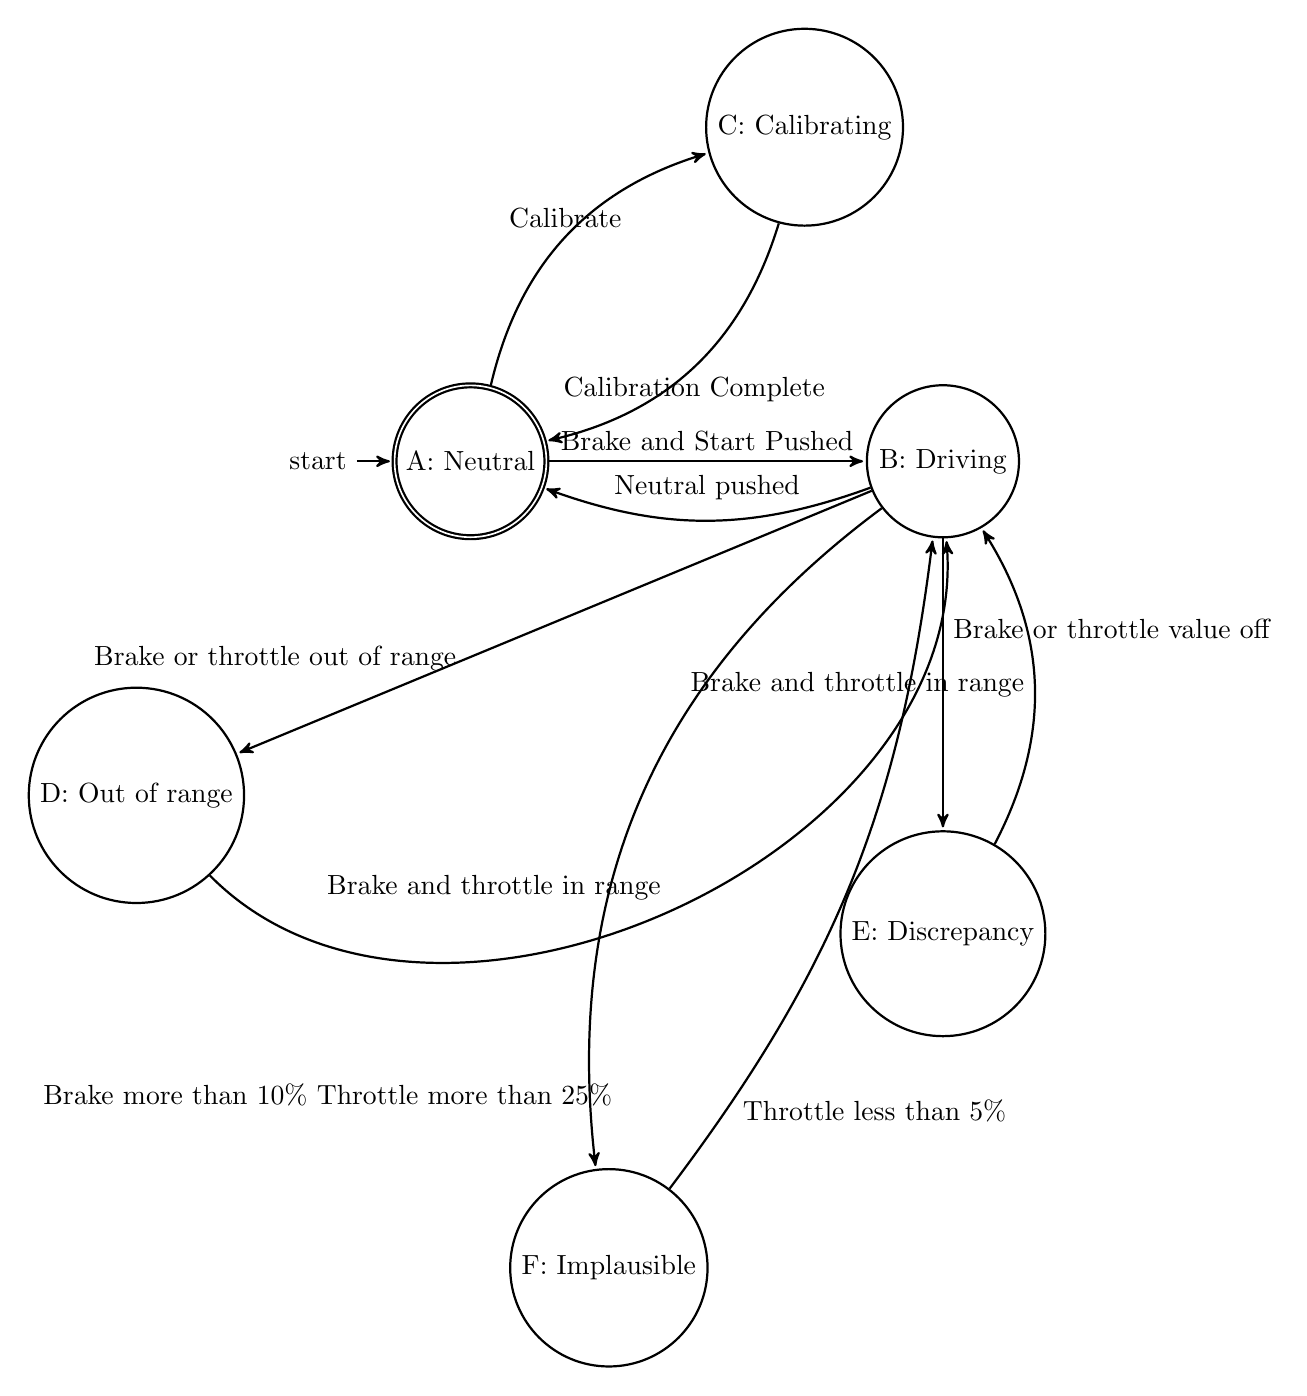
\begin{tikzpicture}[shorten >=1pt,->,>=stealth',shorten >=1pt,auto,node distance=2.8cm,
                    thick, node distance=6cm]
  \tikzstyle{every state}=[fill=white,text=black]

  \node[initial,state, accepting] (A)                    {A: Neutral};
  \node[state]                    (B) [ right of=A] {B: Driving};
  \node[state]                     (C) [above right of=A] {C: Calibrating};
  \node[state]                    (D) [below left of =A] {D: Out of range};
  \node[state]                    (E) [below  of =B] {E: Discrepancy};
  \node[state]                    (F) [below left of =E] {F: Implausible};

  \path (A) edge            node  {Brake and Start Pushed} (B)
            edge [bend left]             node[above] {Calibrate} (C)
        (B) edge [bend left=20]           node[yshift=20pt]  {Neutral pushed} (A)
            edge              node[yshift=20pt] {Brake or throttle value off} (E)
            edge              node[xshift=-170pt, yshift=-5pt] {Brake or throttle out of range} (D)
            edge [bend right]             node[xshift=-220pt, yshift=-100pt] {Brake more than 10\% Throttle more than 25\%} (F)
        (C) edge [bend left]             node[below] {Calibration Complete} (A)
        (D) edge [bend right=70]             node {Brake and throttle in range} (B)
        (E) edge [bend right]             node {Brake and throttle in range} (B)
        (F) edge [bend right=15]             node[xshift=60pt, yshift=-90pt] {Throttle less than 5\%} (B);
\end{tikzpicture}

\end{document}
